% Options for packages loaded elsewhere
\PassOptionsToPackage{unicode}{hyperref}
\PassOptionsToPackage{hyphens}{url}
\PassOptionsToPackage{dvipsnames,svgnames,x11names}{xcolor}
\documentclass[
  10pt,
  fontset=fandol]{ctexart}
\usepackage{xcolor}
\usepackage[margin=16mm]{geometry}
\usepackage{amsmath,amssymb}
\setcounter{secnumdepth}{-\maxdimen} % remove section numbering
\usepackage{iftex}
\ifPDFTeX
  \usepackage[T1]{fontenc}
  \usepackage[utf8]{inputenc}
  \usepackage{textcomp} % provide euro and other symbols
\else % if luatex or xetex
  \usepackage{unicode-math} % this also loads fontspec
  \defaultfontfeatures{Scale=MatchLowercase}
  \defaultfontfeatures[\rmfamily]{Ligatures=TeX,Scale=1}
\fi
\usepackage{lmodern}
\ifPDFTeX\else
  % xetex/luatex font selection
\fi
% Use upquote if available, for straight quotes in verbatim environments
\IfFileExists{upquote.sty}{\usepackage{upquote}}{}
\IfFileExists{microtype.sty}{% use microtype if available
  \usepackage[]{microtype}
  \UseMicrotypeSet[protrusion]{basicmath} % disable protrusion for tt fonts
}{}
\makeatletter
\@ifundefined{KOMAClassName}{% if non-KOMA class
  \IfFileExists{parskip.sty}{%
    \usepackage{parskip}
  }{% else
    \setlength{\parindent}{0pt}
    \setlength{\parskip}{6pt plus 2pt minus 1pt}}
}{% if KOMA class
  \KOMAoptions{parskip=half}}
\makeatother
\usepackage{longtable,booktabs,array}
\newcounter{none} % for unnumbered tables
\usepackage{calc} % for calculating minipage widths
% Correct order of tables after \paragraph or \subparagraph
\usepackage{etoolbox}
\makeatletter
\patchcmd\longtable{\par}{\if@noskipsec\mbox{}\fi\par}{}{}
\makeatother
% Allow footnotes in longtable head/foot
\IfFileExists{footnotehyper.sty}{\usepackage{footnotehyper}}{\usepackage{footnote}}
\makesavenoteenv{longtable}
\usepackage{graphicx}
\makeatletter
\newsavebox\pandoc@box
\newcommand*\pandocbounded[1]{% scales image to fit in text height/width
  \sbox\pandoc@box{#1}%
  \Gscale@div\@tempa{\textheight}{\dimexpr\ht\pandoc@box+\dp\pandoc@box\relax}%
  \Gscale@div\@tempb{\linewidth}{\wd\pandoc@box}%
  \ifdim\@tempb\p@<\@tempa\p@\let\@tempa\@tempb\fi% select the smaller of both
  \ifdim\@tempa\p@<\p@\scalebox{\@tempa}{\usebox\pandoc@box}%
  \else\usebox{\pandoc@box}%
  \fi%
}
% Set default figure placement to htbp
\def\fps@figure{htbp}
\makeatother
\setlength{\emergencystretch}{3em} % prevent overfull lines
\providecommand{\tightlist}{%
  \setlength{\itemsep}{0pt}\setlength{\parskip}{0pt}}
\usepackage{amsmath,amssymb,mathtools,needspace}
\xeCJKDeclareCharClass{CJK}{"2032,"0400->"04FF,"2160->"216B,"2460->"2473,"25A0,"25C7,"25CB,"25CF}
\IfFontExistsTF{Arial Unicode MS}{\xeCJKsetup{AutoFallBack=true}\setCJKfallbackfamilyfont{\CJKrmdefault}{Arial Unicode MS}}{}
\setcounter{secnumdepth}{0}
\setlength{\emergencystretch}{2em}
\allowdisplaybreaks
\usepackage{bookmark}
\IfFileExists{xurl.sty}{\usepackage{xurl}}{} % add URL line breaks if available
\urlstyle{same}
\hypersetup{
  pdftitle={线性多步法},
  colorlinks=true,
  linkcolor={Maroon},
  filecolor={Maroon},
  citecolor={Blue},
  urlcolor={Blue},
  pdfcreator={LaTeX via pandoc}}

\title{线性多步法}
\author{}
\date{}

\begin{document}
\maketitle

\subsection{5.5 线性多步法}\label{ux7ebfux6027ux591aux6b65ux6cd5}

在逐步推进的求解过程中，计算 \(y_{n+1}\) 之前事实上已经求出了一系列的近似值 \(y_n,y_{n-1},y_{n-2},\cdots\)，如果充分利用前面多步的信息来预测 \(y_{n+1}\)，则可以期望会获得较高的精度。这就是构造所谓线性多步法的基本思想。

构造多步法有多种途径，下面介绍其中两种：基于数值积分的构造方法和基于 Taylor 展开的构造方法。

\subsubsection{5.5.1 基于数值积分的构造方法}\label{ux57faux4e8eux6570ux503cux79efux5206ux7684ux6784ux9020ux65b9ux6cd5}

将方程 \(y'=f(x,y)\) 的两端从 \(x_n\) 到 \(x_{n+1}\) 求积分，得

\[
y(x_{n+1})=y(x_n)+\int_{x_n}^{x_{n+1}}f(x,y(x))\,\mathrm dx.
\tag{5.5.1}
\]

为了通过这个积分关系式获得 \(y(x_{n+1})\) 的近似值，只要近似地算出其中的积分项 \(\int_{x_n}^{x_{n+1}}f(x,y(x))\,\mathrm dx\) 即可。选用不同的数值方法计算这个积分项，就会导出不同的计算格式。

例如，设用矩形方法计算积分项，即

\[
\int_{x_n}^{x_{n+1}}f(x,y(x))\,\mathrm dx\approx hf(x_n,y(x_n)),
\]

代入式（5.5.1），有

\[
y(x_{n+1})\approx y(x_n)+hf(x_n,y(x_n)),
\]

据此离散化即可导出 Euler 格式。

\href{../../source-images/pdf-138.jpeg}{原页}

为了改善精度，可以改用梯形方法计算积分项，即

\[
\int_{x_n}^{x_{n+1}}f(x,y(x))\,\mathrm dx\approx\frac h2[f(x_n,y(x_n))+f(x_{n+1},y(x_{n+1}))],
\]

再代入式（5.5.1），有

\[
y(x_{n+1})\approx y(x_n)+\frac h2[f(x_n,y(x_n))+f(x_{n+1},y(x_{n+1}))],
\]

据此离散化即可导出格式（5.2.8），\textbf{梯形法}因此而得名。

我们知道，基于插值原理可以建立一系列的数值积分方法，运用这些方法可以导出求解微分方程的一系列的计算格式。一般地，设已构造出 \(f(x,y(x))\) 的插值多项式 \(P_r(x)\)，那么，计算 \(\int_{x_n}^{x_{n+1}}P_r(x)\,\mathrm dx\) 作为 \(\int_{x_n}^{x_{n+1}}f(x,y(x))\,\mathrm dx\) 的近似值，即可将式（5.5.1）离散化得到下列计算公式：

\[
y_{n+1}=y_n+\int_{x_n}^{x_{n+1}}P_r(x)\,\mathrm dx.
\tag{5.5.2}
\]

\subsubsection{5.5.2 Adams 显式格式}\label{adams-ux663eux5f0fux683cux5f0f}

运用插值方法的关键，在于选取合适的插值节点。记 \(f_k=f(x_k,y_k)\)，先用 \(r+1\) 个数据点 \((x_n,\allowbreak f_n),\allowbreak (x_{n-1},\allowbreak f_{n-1}),\allowbreak \cdots,\allowbreak (x_{n-r},\allowbreak f_{n-r})\) 构造插值多项式 \(P_r(x)\)，注意到这里插值节点 \(x_n,x_{n-1},\cdots,x_{n-r}\) 等距，运用 Newton 后插公式（见 2.4.2 节）可写出

\[
P_r(x_n+th)=\sum_{j=0}^r(-1)^j\binom{-t}{j}\Delta^j f_{n-j},
\]

其中 \(t=\dfrac{x-x_n}{h}\)，\(\Delta^j\) 表示 \(j\) 阶向前差分，而

\[
\binom sj=\frac{s(s-1)\cdots(s-j+1)}{j!}.
\]

将 \(P_r(x)\) 的上述表达式代入式（5.5.2），即得下列 \textbf{Adams 显式格式}

\[
y_{n+1}=y_n+h\sum_{j=0}^r\alpha_j\Delta^j f_{n-j},
\tag{5.5.3}
\]

其中 \(\alpha_j\) 为不依赖于 \(n\) 和 \(r\) 的系数，\(\alpha_j=(-1)^j\int_0^1\binom{-t}{j}\,\mathrm dt\)。它的前几个值如表 5.6 所示。

\textbf{表 5.6}

{\def\LTcaptype{none} % do not increment counter
\begin{longtable}[]{@{}lrrrr@{}}
\toprule\noalign{}
\(j\) & 0 & 1 & 2 & 3 \\
\midrule\noalign{}
\endhead
\bottomrule\noalign{}
\endlastfoot
\(\alpha_j\) & 1 & \(1/2\) & \(5/12\) & \(3/8\) \\
\end{longtable}
}

实际计算时，将格式（5.5.3）中的差分展开往往是方便的，利用差分展开式 \(\Delta^j f_{n-j}=\sum_{i=0}^r(-1)^i\binom ji f_{n-j}\)，可将它改写为

\[
y_{n+1}=y_n+h\sum_{i=0}^r\beta_{ri}f_{n-i},\qquad
\beta_{ri}=(-1)^i\sum_{j=i}^r\binom ji\alpha_j.
\tag{5.5.4}
\]

\begin{quote}
校注（agent 补充）：原图中上述未编号``差分展开式''的求和上限印作 \(r\)，求和项末尾印作 \(f_{n-j}\)，这里均保留原文。末尾下标疑为原书排印错误，通常应为 \(f_{n-i}\)；例如 \(j=r=1\) 时，原印刷式右边为零，而左边为 \(f_n-f_{n-1}\)。按通常写法求和上限为 \(j\)；若约定 \(\binom ji=0\)（\(i>j\)），则上限写 \(r\) 也可。此疑误已对照原页局部图，并非 OCR 替换。
\end{quote}

\href{../../source-images/pdf-139.jpeg}{原页}

这里，系数 \(\beta_{ri}\) 与 \(r\) 的定值有关，其具体数值如表 5.7 所示。式（5.5.4）是含有参数 \(r\) 的一族格式，\(r+1\) 为格式的步数。特别地，一步显式 Adams 格式（\(r=0\)）即为 Euler 格式。两步显式 Adams 格式（\(r=1\)）为

\[
y_{n+1}=y_n+\frac h2(3f_n-f_{n-1}),
\tag{5.5.5}
\]

\textbf{表 5.7}

{\def\LTcaptype{none} % do not increment counter
\begin{longtable}[]{@{}lrrrr@{}}
\toprule\noalign{}
\(i\) & 0 & 1 & 2 & 3 \\
\midrule\noalign{}
\endhead
\bottomrule\noalign{}
\endlastfoot
\(\beta_{0i}\) & 1 & & & \\
\(\beta_{1i}\) & \(3/2\) & \(-1/2\) & & \\
\(\beta_{2i}\) & \(23/12\) & \(-16/12\) & \(5/12\) & \\
\(\beta_{3i}\) & \(55/24\) & \(-59/24\) & \(37/24\) & \(-9/24\) \\
\end{longtable}
}

而四步显式 Adams 格式（\(r=3\)）则为

\[
y_{n+1}=y_n+\frac h{24}(55f_n-59f_{n-1}+37f_{n-2}-9f_{n-3}).
\tag{5.5.6}
\]

\subsubsection{5.5.3 Adams 隐式格式}\label{adams-ux9690ux5f0fux683cux5f0f}

上述 Adams 显式方法选 \(x_n,x_{n-1},\cdots,x_{n-r}\) 作为插值节点，这时，用插值函数 \(P_r(x)\) 在求积区间 \([x_n,x_{n+1}]\) 上逼近 \(f(x,y(x))\)，实际上是个外推过程，效果不够理想。为了改善逼近效果，可以变外推为内插，改用 \(x_{n+1},x_n,\cdots,x_{n-r+1}\) 为插值节点；而通过数据点 \((x_{n+1},\allowbreak f_{n+1}),\allowbreak (x_n,\allowbreak f_n),\allowbreak \cdots,\allowbreak (x_{n-r+1},\allowbreak f_{n-r+1})\) 插出函数 \(P_r(x)\)，然后重复前一段的推导过程。对应于式（5.5.3），这里有下列 \textbf{Adams 隐式格式}：

\[
y_{n+1}=y_n+h\sum_{j=0}^r\alpha_j^*\Delta^j f_{n-j+1},\qquad
\alpha_j^*=(-1)^j\int_{-1}^0\binom{-t}{j}\,\mathrm dt.
\tag{5.5.7}
\]

它的前几个值如表 5.8 所示。

\textbf{表 5.8}

{\def\LTcaptype{none} % do not increment counter
\begin{longtable}[]{@{}lrrrr@{}}
\toprule\noalign{}
\(j\) & 0 & 1 & 2 & 3 \\
\midrule\noalign{}
\endhead
\bottomrule\noalign{}
\endlastfoot
\(\alpha_j^*\) & 1 & \(-1/2\) & \(-1/12\) & \(-1/24\) \\
\end{longtable}
}

\textbf{表 5.9}

{\def\LTcaptype{none} % do not increment counter
\begin{longtable}[]{@{}lrrrr@{}}
\toprule\noalign{}
\(i\) & 0 & 1 & 2 & 3 \\
\midrule\noalign{}
\endhead
\bottomrule\noalign{}
\endlastfoot
\(\beta_{0i}^*\) & 1 & & & \\
\(\beta_{1i}^*\) & \(1/2\) & \(1/2\) & & \\
\(\beta_{2i}^*\) & \(5/12\) & \(8/12\) & \(-1/12\) & \\
\(\beta_{3i}^*\) & \(9/24\) & \(19/24\) & \(-5/24\) & \(1/24\) \\
\end{longtable}
}

将差分展开，式（5.5.7）可改写为

\[
y_{n+1}=y_n+h\sum_{i=0}^r\beta_{ri}^*f_{n-i+1},\qquad
\beta_{ri}^*=(-1)^i\sum_{j=i}^r\binom ji\alpha_j^*.
\tag{5.5.8}
\]

表 5.9 提供了系数 \(\beta_{ri}^*\) 的部分数值。式（5.5.8）是含有参数 \(r\) 的一族格式，\(r+1\) 为格式的步数。特别地，一步隐式 Adams 格式（\(r=0\)）为后退的 Euler 格式。两步隐式 Adams 格式（\(r=1\)）为梯形格式，而四步隐式 Adams 格式（\(r=3\)）则为

\[
y_{n+1}=y_n+\frac h{24}(9f_{n+1}+19f_n-5f_{n-1}+f_{n-2}).
\tag{5.5.9}
\]

\href{../../source-images/pdf-140.jpeg}{原页}

\subsubsection{5.5.4 Adams 预测-校正系统}\label{adams-ux9884ux6d4b-ux6821ux6b63ux7cfbux7edf}

可以同前述 Euler 方法一样分析 Adams 方法的误差。譬如，对于格式（5.5.6），假设 \(y_{n-k}=y(x_{n-k})\)（\(k=0,1,2,3\)），这时

\[
f_{n-k}=f(x_{n-k},y_{n-k})=f(x_{n-k},y(x_{n-k}))=y'(x_{n-k})\qquad(k=0,1,2,3),
\]

代入式（5.5.6），有

\[
y_{n+1}=y(x_n)+\frac h{24}[55y'(x_n)-59y'(x_{n-1})+37y'(x_{n-2})-9y'(x_{n-3})].
\]

将上式右端各项在点 \(x_n\) 展开，得

\[
\begin{aligned}
y_{n+1}={}&y(x_n)+hy'(x_n)+\frac{h^2}{2}y''(x_n)+\frac{h^3}{6}y'''(x_n)\\
&+\frac{h^4}{24}y^{(4)}(x_n)-\frac{49}{144}h^5y^{(5)}(x_n)+\cdots.
\end{aligned}
\]

另一方面，对于准确解 \(y(x_{n+1})\)，有

\[
y(x_{n+1})=y(x_n)+hy'(x_n)+\frac{h^2}{2}y''(x_n)+\frac{h^3}{6}y'''(x_n)+\frac{h^4}{24}y^{(4)}(x_n)+\frac{h^5}{120}y^{(5)}(x_n)+\cdots,
\]

于是显式格式（5.5.6）的局部截断误差为

\[
y(x_{n+1})-y_{n+1}\approx\frac{251}{720}h^5y^{(5)}(x_n).
\tag{5.5.10}
\]

类似地可以导出隐式格式（5.5.9）的局部截断误差为

\[
y(x_{n+1})-y_{n+1}\approx-\frac{19}{720}h^5y^{(5)}(x_n).
\tag{5.5.11}
\]

注意，显式格式（5.5.6）与隐式格式（5.5.9）都具有四阶精度，这两种格式可匹配成下列 Adams \textbf{预测-校正系统}：

预测

\[
\bar y_{n+1}=y_n+\frac h{24}(55f_n-59f_{n-1}+37f_{n-2}-9f_{n-3}),
\tag{5.5.12}
\]

\[
\bar f_{n+1}=f(x_{n+1},\bar y_{n+1});
\]

校正

\[
y_{n+1}=y_n+\frac h{24}(9\bar f_{n+1}+19f_n-5f_{n-1}+f_{n-2}),
\tag{5.5.13}
\]

\[
f_{n+1}=f(x_{n+1},y_{n+1}).
\]

这种预测-校正方法是四步法，用它在计算 \(y_{n+1}\) 时，不但要用到前一步的信息 \(y_n,f_n\)，而且要用到更前三步的信息 \(f_{n-1},f_{n-2},f_{n-3}\)，因此它不是自开始的。实际计算时，必须借助某种单步法，如四阶 Taylor 格式（见 5.3.1 节）或四阶 Runge-Kutta 格式（见 5.3.5 节）为它提供开始值 \(y_1,y_2,y_3\)。

\textbf{例 5.6} 用 Adams 预测-校正系统（5.5.12）、（5.5.13）求解初值问题（5.2.2）。

\textbf{解} 取步长 \(h=0.1\) 计算。用例 5.3 按四阶 Taylor 格式求得的结果 \(y_1,y_2,y_3\) 作为开始值，然后启动格式（5.5.12）、（5.5.13）进行计算。计算结果如表 5.10 所示。表

\href{../../source-images/pdf-141.jpeg}{原页}

（接上页）中 \(\bar y_n\) 和 \(y_n\) 分别为预测值和校正值，同时列出了准确值 \(y(x_n)\) 以比较计算结果的精度。

依据误差公式（5.5.10）和式（5.5.11），对于系统（5.5.12）、（5.5.13）中的预测值 \(\bar y_{n+1}\) 和校正值 \(y_{n+1}\)，分别有

\[
y(x_{n+1})-\bar y_{n+1}\approx\frac{251}{720}h^5y^{(5)}(x_n),
\]

\[
y(x_{n+1})-y_{n+1}\approx-\frac{19}{720}h^5y^{(5)}(x_n).
\]

于是有下列事后估计式：

\[
y(x_{n+1})-\bar y_{n+1}\approx-\frac{251}{720}(\bar y_{n+1}-y_{n+1}),
\]

\[
y(x_{n+1})-y_{n+1}\approx\frac{19}{720}(\bar y_{n+1}-y_{n+1}).
\]

\textbf{表 5.10}

{\def\LTcaptype{none} % do not increment counter
\begin{longtable}[]{@{}lrrr@{}}
\toprule\noalign{}
\(x_n\) & \(\bar y_n\) & \(y_n\) & \(y(x_n)\) \\
\midrule\noalign{}
\endhead
\bottomrule\noalign{}
\endlastfoot
0 & & 1 & 1 \\
0.1 & & 1.0954 & 1.0954 \\
0.2 & & 1.1832 & 1.1832 \\
0.3 & & 1.2649 & 1.2649 \\
0.4 & 1.3415 & 1.3416 & 1.3416 \\
0.5 & 1.4141 & 1.4142 & 1.4142 \\
0.6 & 1.4832 & 1.4832 & 1.4832 \\
0.7 & 1.5491 & 1.5492 & 1.5492 \\
0.8 & 1.6125 & 1.6125 & 1.6125 \\
0.9 & 1.6734 & 1.6734 & 1.6733 \\
1.0 & 1.7321 & 1.7321 & 1.7231 \\
\end{longtable}
}

利用这一结果，可将 Adams 预测-校正系统（5.5.12）、（5.5.13）进一步加工成下列计算方案：

预测

\[
p_{n+1}=y_n+\frac h{24}(55y'_n-59y'_{n-1}+37y'_{n-2}-9y'_{n-3}),
\]

改进

\[
m_{n+1}=p_{n+1}+\frac{251}{720}(c_n-p_n),
\]

计算

\[
m_{n+1}=f(x_{n+1},m_{n+1}),
\]

校正

\[
c_{n+1}=y_n+\frac h{24}(9m'_{n+1}+19y'_n-5y'_{n-1}+y'_{n-2}),
\]

改进

\[
y_{n+1}=c_{n+1}-\frac{19}{720}(c_{n+1}-p_{n+1}),
\]

计算

\[
y'_{n+1}=f(x_{n+1},y_{n+1}).
\]

关于这种计算方案，读者可参看 5.2 节末的有关论述。

\subsubsection{5.5.5 基于 Taylor 展开的构造方法}\label{ux57faux4e8e-taylor-ux5c55ux5f00ux7684ux6784ux9020ux65b9ux6cd5}

我们看到，基于数值积分可以构造出一系列求解常微分方程的计算格式，然而下面将要介绍的 Taylor 展开方法更具有一般性，各种线性多步格式（包括前述 Adams 格式）均可通过这种方法构造出来。

一般的线性多步格式具有下列形式：

\[
y_{n+1}=\alpha_0y_n+\alpha_1y_{n-1}+\cdots+\alpha_ry_{n-r}+h(\beta_{-1}y'_{n+1}+\beta_0y'_n+\beta_1y'_{n-1}+\cdots+\beta_ry'_{n-r}),
\]

缩记作

\begin{quote}
校注（agent 补充，ch05b-E002）：本页两条``事后估计式''及计算方案两条``改进''式的分母均印为 \(720\)，已照录。由本页前两条局部误差式相减，\(y_{n+1}-\bar y_{n+1}\approx(270/720)h^5y^{(5)}(x_n)\)，消去 \(h^5y^{(5)}(x_n)\) 后，事后估计的系数应为 \(251/270\) 和 \(19/270\)；相应改进式中的分母也应为 \(270\)。这是原书疑误，非 OCR 错。

校注（agent 补充，ch05b-E003）：计算方案第一条``计算''式左端印为 \(m_{n+1}\)，未带撇号；已照录。按下一条校正式使用的 \(m'_{n+1}\) 及导数定义，此处疑漏印撇号，应为 \(m'_{n+1}=f(x_{n+1},m_{n+1})\)。

校注（agent 补充，ch05b-E004）：表 5.10 末行准确值原印为 \(1.7231\)，已照录。已另行目视核对 PDF 120（书 107 页）式（5.2.2）后所列解析解 \(y=\sqrt{1+2x}\) 及表 5.1；\(y(1)=\sqrt3\approx1.7321\)，因此本格疑有数字对调。
\end{quote}

\href{../../source-images/pdf-142.jpeg}{原页}

\[
y_{n+1}=\sum_{k=0}^r\alpha_ky_{n-k}+h\sum_{k=-1}^r\beta_ky'_{n-k},
\tag{5.5.14}
\]

其中 \(y'_{n-k}=f(x_{n-k},y_{n-k})\)。注意到 \(y'_{n+1}=f(x_{n+1},y_{n+1})\) 中含有未知的 \(y_{n+1}\)，则当 \(\beta_{-1}=0\) 时，格式（5.5.14）是显式的，\(\beta_{-1}\ne0\) 时则是隐式的。

设 \(y_{n-k}=y(x_{n-k}),y'_{n-k}=y'(x_{n-k})\)，由 Taylor 展开，有

\[
y_{n-k}=\sum_{j=0}^p\frac{(-kh)^j}{j!}y_n^{(j)}+\frac{(-kh)^{p+1}}{(p+1)!}y_n^{(p+1)}+\cdots,
\]

\[
y'_{n-k}=\sum_{j=1}^p\frac{(-kh)^{j-1}}{(j-1)!}y_n^{(j)}+\frac{(-kh)^p}{p!}y_n^{(p+1)}+\cdots.
\]

代入式（5.5.14），整理得

\[
\begin{aligned}
y_{n+1}={}&\left(\sum_{k=0}^r\alpha_k\right)y_n+\sum_{j=1}^p\frac{h^j}{j!}\left[\sum_{k=1}^r(-k)^j\alpha_k+j\sum_{k=-1}^r(-k)^{j-1}\beta_k\right]y_n^{(j)}\\
&+\frac{h^{p+1}}{(p+1)!}\left[\sum_{k=1}^r(-k)^{p+1}\alpha_k+(p+1)\sum_{k=-1}^r(-k)^p\beta_k\right]y_n^{(p+1)}+\cdots.
\end{aligned}
\tag{5.5.15}
\]

于是，欲使格式（5.5.14）成为 \(p\) 阶精度的，即局部截断误差为 \(O(h^{p+1})\)，只要令展开式（5.5.15）与 \(y(x_{n+1})\) 的 Taylor 展开式

\[
y(x_{n+1})=\sum_{j=0}^p\frac{h^j}{j!}y_n^{(j)}+\frac{h^{p+1}}{(p+1)!}y_n^{(p+1)}+\cdots
\tag{5.5.16}
\]

能符合到 \(h^p\) 项，为此要求成立

\[
\begin{cases}
\displaystyle\sum_{k=0}^r\alpha_k=1,\\[6pt]
\displaystyle\sum_{k=1}^r(-k)^j\alpha_k+j\sum_{k=-1}^r(-k)^{j-1}\beta_k=1\qquad(j=1,2,\cdots,p).
\end{cases}
\tag{5.5.17}
\]

如果格式（5.5.14）的系数满足这组条件，则将式（5.5.16）与式（5.5.15）相减，即得局部截断误差

\[
\begin{aligned}
&y(x_{n+1})-y_{n+1}\\
&=\frac{h^{p+1}}{(p+1)!}\left[1-\sum_{k=1}^r(-k)^{p+1}\alpha_k-(p+1)\sum_{k=-1}^r(-k)^p\beta_k\right]y_n^{(p+1)}+\cdots.
\end{aligned}
\tag{5.5.18}
\]

下面进一步具体地考察四步方法。先研究下列形式的四步显式格式：

\[
y_{n+1}=\alpha_0y_n+\alpha_1y_{n-1}+\alpha_2y_{n-2}+h(\beta_0y'_n+\beta_1y'_{n-1}+\beta_2y'_{n-2}+\beta_3y'_{n-3}),
\tag{5.5.19}
\]

欲使这类格式成为四阶的，按式（5.5.17），其系数应当满足条件

\[
\begin{cases}
\alpha_0+\alpha_1+\alpha_2=1,\\
-\alpha_1-2\alpha_2+\beta_0+\beta_1+\beta_2+\beta_3=1,\\
\alpha_1+4\alpha_2-2\beta_1-4\beta_2-6\beta_3=1,\\
-\alpha_1-8\alpha_2+3\beta_1+12\beta_2+27\beta_3=1,\\
\alpha_1+16\alpha_2-4\beta_1-32\beta_2-108\beta_3=1.
\end{cases}
\tag{5.5.20}
\]

\href{../../source-images/pdf-143.jpeg}{原页}

这里有七个待定系数 \(\alpha_0,\allowbreak \alpha_1,\allowbreak \alpha_2,\allowbreak \beta_0,\allowbreak \beta_1,\allowbreak \beta_2,\allowbreak \beta_3\)，然而它们所要适合的条件只有五个，因此有两个自由度。设令 \(\alpha_1=\alpha_2=0\)，求解式（5.5.20）得到

\[
\alpha_0=1,\quad\beta_0=\frac{55}{24},\quad\beta_1=-\frac{59}{24},\quad\beta_2=\frac{37}{24},\quad\beta_3=-\frac9{24}.
\]

这时式（5.5.19）为四阶 Adams 格式（5.5.6）。另外，用定出的系数值具体地代入式（5.5.18），即可导出误差公式（5.5.10）。

为了提供与式（5.5.19）相匹配的隐式方法，舍弃其中的 \(y'_{n-3}\) 而代之以 \(y'_{n+1}\)，有

\[
y_{n+1}=\alpha_0y_{n+1}\alpha_1y_{n-1}+\alpha_2y_{n-2}+h(\beta_{-1}y'_{n+1}+\beta_0y'_n+\beta_1y'_{n-1}+\beta_2y'_{n-2}).
\tag{5.5.21}
\]

为使这类格式具有四阶精度，按式（5.5.17），系数应当满足条件

\[
\begin{cases}
\alpha_0+\alpha_1+\alpha_2=1,\\
-\alpha_1-2\alpha_2+\beta_{-1}+\beta_0+\beta_1+\beta_2=1,\\
\alpha_1+4\alpha_2+2\beta_{-1}-2\beta_1-4\beta_2=1,\\
-\alpha_1-8\alpha_2+3\beta_{-1}+3\beta_1+12\beta_2=1,\\
\alpha_1+16\alpha_2+4\beta_{-1}-4\beta_1-32\beta_2=1.
\end{cases}
\tag{5.5.22}
\]

特别地，取 \(\alpha_1=\alpha_2=0\) 即得四阶 Adams 格式（5.5.9），通过这一途径同时可以导出误差公式（5.5.11）。

\subsubsection{5.5.6 Milne 格式}\label{milne-ux683cux5f0f}

与格式（5.5.19）不同的另一类格式是用 \(y_{n-3}\) 而不用 \(y'_{n-3}\)，其形式为

\[
y_{n+1}=\alpha_0y_n+\alpha_1y_{n-1}+\alpha_2y_{n-2}+\alpha_3y_{n-3}+h(\beta_0y'_n+\beta_1y'_{n-1}+\beta_2y'_{n-2}).
\tag{5.5.23}
\]

类似于前面的讨论，运用 Taylor 展开方法不难导出形如式（5.5.23）的一类四阶方法。这类方法中包含有著名的 Milne 格式

\[
y_{n+1}=y_{n-3}+\frac{4h}{3}(2y'_n-y'_{n-1}+2y'_{n-2}),
\tag{5.5.24}
\]

其局部截断误差为

\[
y(x_{n+1})-y_{n+1}\approx\frac{14}{45}h^5y_n^{(5)}.
\tag{5.5.25}
\]

Milne 格式也可以通过数值积分的途径推导出来。事实上，从积分恒等式

\[
y(x_{n+1})=y(x_{n-3})+\int_{x_{n-3}}^{x_{n+1}}y'(x)\,\mathrm dx
\tag{5.5.26}
\]

着手，用数据点 \((x_n,\allowbreak y'_n),\allowbreak (x_{n-1},\allowbreak y'_{n-1}),\allowbreak (x_{n-2},\allowbreak y'_{n-2})\) 插出二次式 \(P_2(x)\)，然后用 \(P_2(x)\) 替代 \(y'(x)\) 计算式（5.5.26）中的积分项，即可得到上述格式（5.5.24）。

再在形如式（5.5.21）的四阶隐式方法中适当挑选一个与 Milne 格式相匹配。在式（5.5.22）中令 \(\alpha_1=1,\alpha_2=0\)，可定出下列四阶格式：

\begin{quote}
校注（agent 补充，ch05b-E005）：式（5.5.21）右端开头在原图中印作 \(\alpha_0y_{n+1}\alpha_1y_{n-1}\)（``\(+1\)''下沉至下标位置，且两项之间无正常加号），上式按可见字形保留。由本页``舍弃 \(y'_{n-3}\) 而代之以 \(y'_{n+1}\)''及式（5.5.19）、（5.5.22），此处疑为排印错误，预期应是 \(\alpha_0y_n+\alpha_1y_{n-1}\)。局部原图如下，仅用于保存这一排印疑误的可审计证据。
\end{quote}

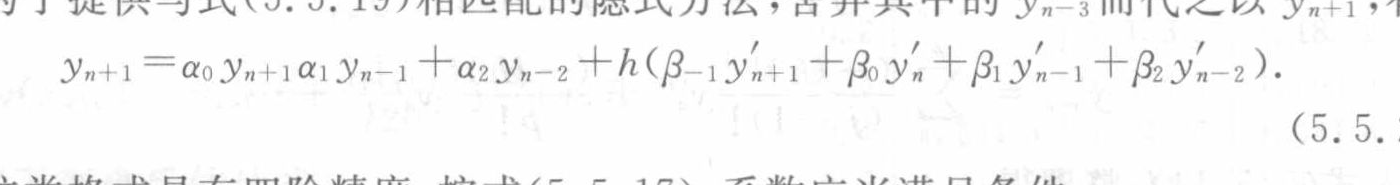
\includegraphics[width=0.85\linewidth,height=\textheight,keepaspectratio,alt={式（5.5.21）原图局部：右端开头的下标与加号排印异常}]{../assets/ch05b/pdf-143-eq521.png}

\href{../../source-images/pdf-144.jpeg}{原页}

\[
y_{n+1}=y_{n-1}+\frac h3(y'_{n+1}+4y'_n+y'_{n-1}).
\tag{5.5.27}
\]

上述格式通常称为 Simpson 格式，用数值积分的 Simpson 方法处理积分恒等式

\[
y(x_{n+1})=y(x_{n-1})+\int_{x_{n-1}}^{x_{n+1}}y'(x)\,\mathrm dx
\]

即可导出这一格式。

用 Simpson 格式（5.5.27）与 Milne 格式（5.5.24）匹配，构成下列预测-校正系统：

预测

\[
\bar y_{n+1}=y_{n-3}+\frac{4h}{3}(2y'_n-y'_{n-1}+2y'_{n-2}),\qquad
\bar y'_{n+1}=f(x_{n+1},\bar y_{n+1});
\]

校正

\[
y_{n+1}=y_{n-1}+\frac h3(\bar y'_{n+1}+4y'_n+y'_{n-1}),\qquad
y'_{n+1}=f(x_{n+1},y_{n+1}).
\]

\subsubsection{5.5.7 Hamming 格式}\label{hamming-ux683cux5f0f}

上述预测-校正系统的缺点是稳定性差。为了改善稳定性，重新挑选校正公式。为此考察式（5.5.21）中不显含 \(y'_{n-2}\) 的一类格式

\[
y_{n+1}=\alpha_0y_n+\alpha_1y_{n-1}+\alpha_2y_{n-2}+h(\beta_{-1}y'_{n+1}+\beta_0y'_n+\beta_1y'_{n-1}),
\tag{5.5.28}
\]

按条件（5.5.22），形如式（5.5.28）的四阶格式含有一个自由度------譬如可取 \(\alpha_1\) 为独立参数。若取 \(\alpha_1=1\) 即得 Simpson 格式（5.5.27）。

Hamming 用 \(\alpha_1\) 的不同数值进行试验，发现当 \(\alpha_1=0\) 时格式的稳定性能较好，即

\[
y_{n+1}=\frac18(9y_n-y_{n-2})+\frac{3h}{8}(y'_{n+1}+2y'_n-y'_{n-1}),
\tag{5.5.29}
\]

其局部截断误差为

\[
y(x_{n+1})-y_{n+1}\approx-\frac{h^5}{40}y_n^{(5)}.
\tag{5.5.30}
\]

Hamming 格式（5.5.29）不能用数值积分方法推导出来。

用 Milne 格式（5.5.24）与 Hamming 格式（5.5.29）相匹配，并利用误差公式（5.5.25）、（5.5.30）改进计算结果，即可建立下列预测-校正系统：

预测

\[
p_{n+1}=y_{n-3}+\frac{4h}{3}(2y'_n-y'_{n-1}+2y'_{n-2}),
\]

改进

\[
m_{n+1}=p_{n+1}-\frac{112}{121}(p_n-c_n),
\]

计算

\[
m'_{n+1}=f(x_{n+1},m_{n+1}),
\]

校正

\[
c_{n+1}=\frac18(9y_n-y_{n-2})+\frac{3h}{8}(m'_{n+1}+2y'_n-y'_{n-1}),
\]

改进

\[
y_{n+1}=c_{n+1}+\frac9{121}(p_{n+1}-c_{n+1}),
\]

\href{../../source-images/pdf-145.jpeg}{原页}

计算

\[
y'_{n+1}=f(x_{n+1},y_{n+1}).
\]

\subsection{本节覆盖原页的校注记录}\label{ux672cux8282ux8986ux76d6ux539fux9875ux7684ux6821ux6ce8ux8bb0ux5f55}

下列记录按原页关联，含同页相邻小节的校注；计算时同时读取上文校注和完整原页。

\begin{itemize}
\tightlist
\item
  \texttt{ch05b-E001}：原书 PDF 页 138
\item
  \texttt{ch05b-E002}：原书 PDF 页 141
\item
  \texttt{ch05b-E003}：原书 PDF 页 141
\item
  \texttt{ch05b-E004}：原书 PDF 页 141
\item
  \texttt{ch05b-E005}：原书 PDF 页 143
\end{itemize}

\end{document}
